\documentclass{article}

\usepackage{fancyhdr}
\usepackage{extramarks}
\usepackage{amsmath}
\usepackage{amsthm}
\usepackage{amsfonts}
\usepackage{tikz}
\usepackage[plain]{algorithm}
\usepackage{algpseudocode}
\usepackage{enumitem}
\usetikzlibrary{automata,positioning}
\usepackage[T1]{fontenc}
\usepackage{textcomp}
\usepackage{listings}
\usepackage{xcolor}
\usepackage{blindtext}
\usepackage{multicol}
\setlength{\columnsep}{1cm}

\lstset{
 language=caml,
 columns=[c]fixed,
% basicstyle=\small\ttfamily,
 keywordstyle=\bfseries,
 upquote=true,
 commentstyle=,
 breaklines=true,
 showstringspaces=false,
 stringstyle=\color{blue},
 literate={'"'}{\textquotesingle "\textquotesingle}3
}

%
% Basic Document Settings
%

\topmargin=-0.45in
\evensidemargin=0in
\oddsidemargin=0in
\textwidth=6.5in
\textheight=9.0in
\headsep=0.25in

\linespread{1.1}

\pagestyle{fancy}
\lhead{\hmwkAuthorName}
\chead{\hmwkClass: \hmwkTitle}
\rhead{\firstxmark}
\lfoot{\lastxmark}
\cfoot{\thepage}

\renewcommand\headrulewidth{0.4pt}
\renewcommand\footrulewidth{0.4pt}

\setlength\parindent{0pt}

%
% Create Problem Sections
%

\newcommand{\enterProblemHeader}[1]{
    \nobreak\extramarks{}{Problem \arabic{#1} continued on next page\ldots}\nobreak{}
    \nobreak\extramarks{Problem \arabic{#1} (continued)}{Problem \arabic{#1} continued on next page\ldots}\nobreak{}
}

\newcommand{\exitProblemHeader}[1]{
    \nobreak\extramarks{Problem \arabic{#1} (continued)}{Problem \arabic{#1} continued on next page\ldots}\nobreak{}
    \stepcounter{#1}
    \nobreak\extramarks{Problem \arabic{#1}}{}\nobreak{}
}

\setcounter{secnumdepth}{0}
\newcounter{partCounter}
\newcounter{homeworkProblemCounter}
\setcounter{homeworkProblemCounter}{1}

%
% Homework Problem Environment
%
% This environment takes an optional argument. When given, it will adjust the
% problem counter. This is useful for when the problems given for your
% assignment aren't sequential. See the last 3 problems of this template for an
% example.
%
\newenvironment{homeworkProblem}[1][-1]{
    \ifnum#1>0
        \setcounter{homeworkProblemCounter}{#1}
    \fi
    \section{Problem \arabic{homeworkProblemCounter}}
    \setcounter{partCounter}{1}
    \enterProblemHeader{homeworkProblemCounter}
}{
    \exitProblemHeader{homeworkProblemCounter}
}

%
% Homework Details
%   - Title
%   - Due date
%   - Class
%   - Section/Time
%   - Instructor
%   - Author
%

\newcommand{\hmwkTitle}{Homework\ \#3}
\newcommand{\hmwkDueDate}{November 14, 2021}
\newcommand{\hmwkClass}{Programming Languages}
\newcommand{\hmwkClassInstructor}{Professor Christian Skalka}
\newcommand{\hmwkAuthorName}{\textbf{Vincent Moeykens}}

%
% Title Page
%

\title{
    \vspace{2in}
    \textmd{\textbf{\hmwkClass:\ \hmwkTitle}}\\
    \normalsize\vspace{0.1in}\small{Due\ on\ \hmwkDueDate}\\
    \vspace{0.1in}\large{\textit{\hmwkClassInstructor}}
    \vspace{3in}
}

\author{\hmwkAuthorName}
\date{}

\renewcommand{\part}[1]{\textbf{\large Part \Alph{partCounter}}\stepcounter{partCounter}\\}

%
% Various Helper Commands
%

% Useful for algorithms
\newcommand{\alg}[1]{\textsc{\bfseries \footnotesize #1}}

% For derivatives
\newcommand{\deriv}[1]{\frac{\mathrm{d}}{\mathrm{d}x} (#1)}

% For partial derivatives
\newcommand{\pderiv}[2]{\frac{\partial}{\partial #1} (#2)}

% Integral dx
\newcommand{\dx}{\mathrm{d}x}

% Alias for the Solution section header
\newcommand{\solution}{\textbf{\large Solution}}

% Probability commands: Expectation, Variance, Covariance, Bias
\newcommand{\E}{\mathrm{E}}
\newcommand{\Var}{\mathrm{Var}}
\newcommand{\Cov}{\mathrm{Cov}}
\newcommand{\Bias}{\mathrm{Bias}}

\begin{document}

% \maketitle

\pagebreak

\begin{homeworkProblem}
    \textbf{Question:} Provide a screen shot of the OCaml editor and interpreter combination you are using for the class.


    \textbf{Solution:} I am using the Vim editor and the \verb|utop| interpreter. \\

	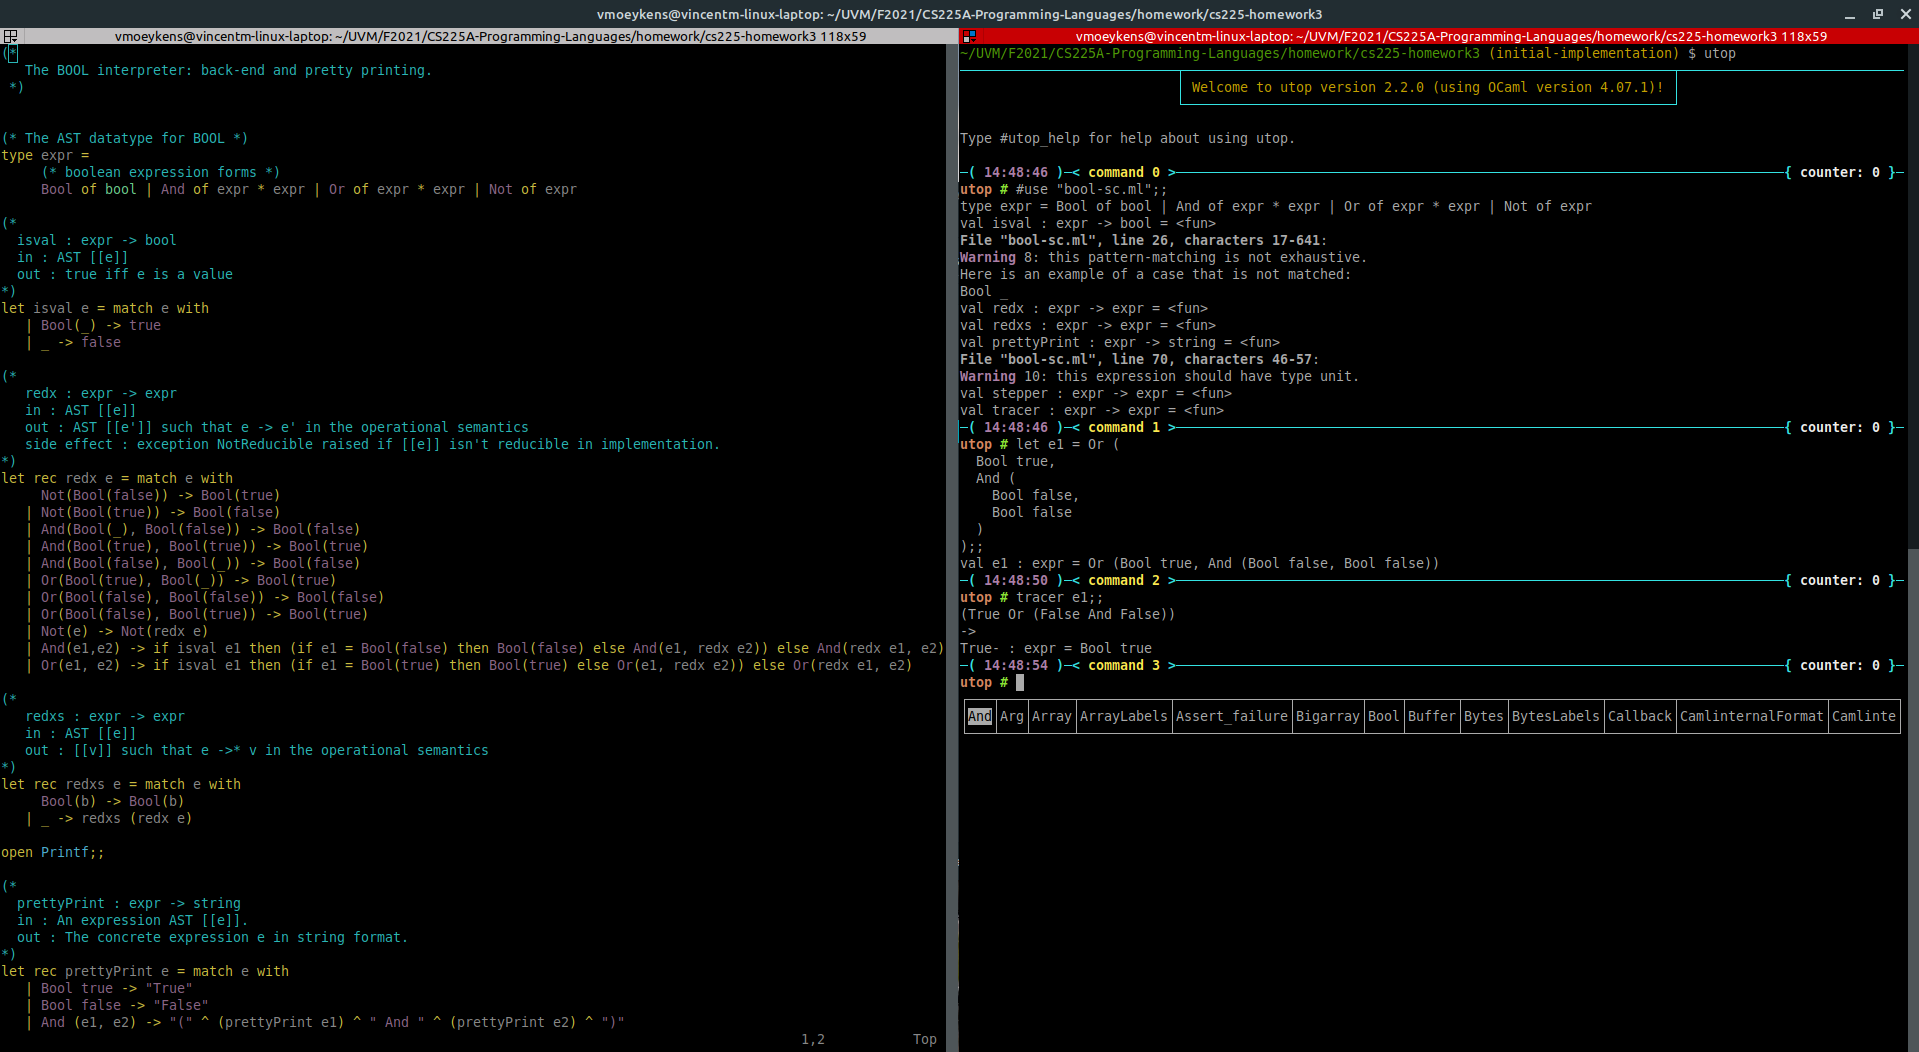
\includegraphics[scale=0.25]{workflow_screenshot_2.png}
	
\end{homeworkProblem}
% ---------------------------------------------------------------------------------- %
\begin{homeworkProblem}
    \textbf{Question:}
Recall that in OCaml, record fields can be constructed from expressions that need to be evaluated. For example, given: \verb|type rt = { a : int; b : int }| we have: \verb|{ a = 1 + 2; b = 3 * 7 }| $\Downarrow$ \verb|{ a = 3; b = 21 }| and it must be the case that either 1 + 2 is evaluated before 3 * 7 or vice-versa in any given implementation. Show which is the case on yours by devising an example that reveals it, and copy-paste or provide a screenshot of your interaction with the interpreter that demonstrates the evidence.\\


    \textbf{Solution:}
    The following code helps demonstrate that the record constructor evaluates right to left. We utilze a reference and a method that takes an integer argument, adds that argument to the current record value, and then returns the record value itself. We then use this method as the value when constructing our record, and we can see that if there was a left to right evaluation order, \verb|a| would be set to \verb|1| since \verb|se| begins as 0, and then \verb|b| would subsequently be set to \verb|3|.
     \begin{lstlisting}
		let se = ref 0;;
		type rt = { a : int; b : int };;
		let inc x = (se := (x + !se); !se);;
		{ a = inc 1; b = inc 2; };;
 	\end{lstlisting}
 	
 	Instead, the output we get from the above OCaml code is the following: \\
 	\verb|- : rt = {a = 3; b = 2}|\\
 	This shows us that \verb|b| is evaluated first, and sets the record to 2, and then \verb|a| is evaluated, and is set to 3.

\end{homeworkProblem}
% ---------------------------------------------------------------------------------- %
\begin{homeworkProblem}
    \textbf{Question:} Suppose you wanted to add an xor operation as a primitive to BOOL. To accomplish this, do the following: \\
    a. Propose a symbol for xor and extend the BOOL language of expressions to admit it as a binary operation\\
    b. Extend the computational and contextual reduction rules of BOOL to provide an operational semantics for xor. You can specify either a left-to-right or right-to-left reduction semantics, but your semantics should be deterministic in the sense of Lecture Notes 9, Proposition 1.1.\\

    \textbf{Solution:}
		\begin{enumerate}[label=\alph*.]
			\item The proposed symbol for xor is "Xor". The new BOOL:
				\begin{align*}
					v &\quad::= \text{True | False} &\quad values \\
					e &\quad::= v \text{ | }e \text{ And } e \text{ | } e \text{ Or } e \text{ | } \text{ Not } e \text{ | } (e) \text{ | } e\text{ Xor } e&\quad expressions \\
				\end{align*}
			\item Our additional computational rules are as follows:
				\begin{align*}
					\textbf{Xor1} &\quad \textbf{Xor2}  \\
					\text{True Xor False}\rightarrow\text{True} &\quad \text{False Xor True}\rightarrow\text{True}
				\end{align*}
				\begin{align*}
					\textbf{Xor3} &\quad \textbf{Xor4} \\
					\text{False Xor False}\rightarrow\text{False} &\quad \text{True Xor True}\rightarrow\text{False}
				\end{align*}
				Our additional contextual rules are as follows:
				\begin{align*}
					\textbf{XorCL} &\quad \textbf{XorCR}  \\
					\frac{e_1\rightarrow e_1'}{e_1\text{ Xor }e_2\rightarrow e_1'\text{ Xor }e_2} &\quad \frac{e\rightarrow e'}{v\text{ Xor }e\rightarrow v\text{ Xor }e'}
				\end{align*}
		\end{enumerate}
\end{homeworkProblem}
% ---------------------------------------------------------------------------------- %
\begin{homeworkProblem}
    \textbf{Question:} Is your modified interpreter still correct in the sense of Lecture Notes 10, Theorem 1.1? If you say no, provide an example that illustrates the fallacy.

    \textbf{Solution:} Yes, the modified interpreter is still correct according to Theorem 1.1. This is because we can still generate a new expression from \verb|redx| if the expression would normall reduce to another expression. Similarly, we can still reduce any expression to a value with any number of steps using \verb|redxs| if the expression would have reduced to a value. 

\end{homeworkProblem}

% ---------------------------------------------------------------------------------- %
\end{document}

